\documentclass{UoYCSproject}
\usepackage{graphicx}
\usepackage[nottoc,numbib]{tocbibind}
\usepackage{subcaption}
\usepackage{listings}
\usepackage{wrapfig}

\usepackage[utf8]{inputenc}
\usepackage[acronym]{glossaries}

\addbibresource{Report.bib}
\title{Parallel Programming Tools for Exploring Immune System Development}
\author{Oliver Binns}
\MEng
\date{\today}
\supervisor{Dr. Fiona Polack, Dr. Kieran Alden}
\wordcount{6007}


%Approx 500 Words
\abstract{
More powerful computers are paving the way for sophisticated simulations of previously underexplored complex biological systems.
\acrlong{abm} has been previously used to implement this type of simulation, showing how the behaviour of a number of individual agents can contribute to the system as a whole.

As advancements in computing tend towards parallelism and distributed systems, these increasingly elaborate simulations must take full advantage of this change in order to be computed in a reasonable time period.
Creating programs and simulations that make efficient use of this parallelism can be technically challenging. In particular it requires implementing an optimal distribution of tasks over the system and ensuring the integrity of any memory that is shared across multiple threads.
Some significant problems, including a substantial computer science skills shortage, are slowing down the rate of progress in this area.

In this project 
the \gls{FLAME GPU} framework is used to help mitigate some of the difficulties with implementing parallel programs, in order to build on an existing sequential \gls{MASON} simulation.
During the building of the simulation, I have discovered that it is not trivial to compare between the old and new implementations, due to differences in the frameworks used.
For this reason, the final comparison will be done directly to the domain model itself.

Finally, I also propose \gls{mde} as a potential short-term solution to the skills shortage, exploring some of the current \gls{mde} technologies for creating simulations and proposing further advancements to these tools for the future.
These engineering techniques help to clearly show how the simulation is derived from the initial biological domain model. 
%add a little bit about the experiments you have carried out (very brief)
%and a general account of the significant findings (including any drawbacks)
}

\acknowledgements{I would like to my supervisors, Fiona Polack and Kieran Alden, for their support and guidance throughout this project. I would also like to thank the \gls{FLAME GPU} development team at the University of Sheffield for their help in utilising the latest and pre-released features of this framework.}

\makeglossaries
\newacronym{abm}{ABM}{Agent-Based Modelling}
\newacronym{cosmos}{CoSMoS}{Complex Systems Modelling and Simulation Infrastructure}
\newacronym{cpu}{CPU}{Central Processsing Unit}
\newacronym{cuda}{CUDA}{Compute Unified Device Architecture}
\newacronym{evl}{EVL}{Epsilon Validation Language}
\newacronym{egl}{EGL}{Epsilon Generation Language}
\newacronym{flame}{FLAME}{Flexible Large Scale Agent Modelling Environment}
\newacronym{flamegpu}{FLAME GPU}{\acrshort{flame} for the \acrshort{gpu}}
\newacronym{gpu}{GPU}{Graphics Processing Unit}
\newacronym{gpgpu}{GPGPU}{General Purpose \acrshort{gpu} programming}
\newacronym{lto}{LTo}{Lymphoid Tissue organiser cell}
\newacronym{ltin}{LTin}{Lymphoid Tissue initiator cell}
\newacronym{lti}{LTi}{Lymphoid Tissue inducer cell}
\newacronym{mason}{MASON}{Multi-Agent Simulator Of Neighborhoods}
\newacronym{mde}{MDE}{Model-Driven Engineering}

%behavioural model
%complex meaning
\newglossaryentry{FLAME GPU}
{
    name=\glslink{flamegpu}{FLAME GPU},
    description={An extension of the \acrshort{flame} framework which uses \acrshort{gpu}s for parallelism}
}
\newglossaryentry{Host}
{
    name=Host,
    description={In \acrshort{gpgpu} programming, the computer containing the \acrshort{gpu} is referred to as the host}
}
\newglossaryentry{Device}
{
    name=Device,
    description={In \acrshort{gpgpu} programming, the \acrshort{gpu} hardware being used, is referred to as the device}
}
\newglossaryentry{PP}
{
    name=Peyer's Patch,
    description={Clusters of cells that form in the small intestine}
}
\newglossaryentry{LTo}
{
    name=\glslink{lto}{LTo},
    description={A static cell}
}
\newglossaryentry{LTin}
{
    name=\glslink{ltin}{LTin},
    description={A moving cell that can bind to any static cell}
}
\newglossaryentry{LTi}
{
    name=\glslink{lti}{LTi},
    description={}
}
\newglossaryentry{Chemokine}
{
    name=LTo,
    description={Scientific tests conducted using computer simulation}
}
\newglossaryentry{MASON}
{
    name=\glslink{mason}{MASON},
    description={A Java framework for producting simulations using \acrshort{abm}}
}
\newglossaryentry{in-silico}
{
    name=in-silico,
    description={Scientific tests conducted using computer simulation}
}
\newglossaryentry{in-vitro}
{
    name=in-vitro,
    description={Scientific tests conducted using real biological systems under laboratory conditions}
}


\begin{document}
\maketitle
\listoffigures
\listoftables
\printglossary[type=\acronymtype]
\printglossary


%Approx 1000 words
\chapter{Introduction}
%TELL THEM WHAT YOU WILL TELL THEM
%LIT REVIEW: TELL THEM
%RESULTS/EVAL: TELL THEM WHAT YOU TOLD THEM!

Agent-Based Modelling has given good results
%compare to mathematical models?
but can take a long time to run, as simulations become more and more complex.
\\

Here, and throughout this report, complexity does not necessarily refer to simulations that contains several components that are difficult to engineer.
Rather, we discuss simulations that are made up of lots of simple components that interact with each other and the environment in such a way that the system behaviour is so elaborate that it can only be predicted by running the simulation.
\\
%an introduction to what is to follow
%the abstract can be very specific
%Here: a bit more general (i.e. MDE and simulation concerns in general)

\section{Motivation}
%What can be gained from better modelling.. particularly biology..?
%Presentation- see justification slides!
The motivation behind this project is the new knowledge that could be gained from the ability to create efficient parallel biological simulations more easily.
While many biological systems can not be fully studied \gls{in-vitro}, simulations can provide a valid alternative.
%rephrase this--->
Indeed previous work has been used to prove some hypotheses wrong.
%do we need citations/examples here if we are going to discuss this in more detail later on?
%is it ok to reference a later chapter?

%outside of biological exploration, new understanding can..?
This type of \gls{in-silico} experimentation could significantly improve the process by which drugs are developed.
Extensive \gls{in-silico} testing can be performed much more quickly than the current \gls{in-vitro} testing, reducing the time it takes to research new drugs and cures.
Drugs and cures would be available for patients earlier, saving many lives.
Additionally, the significant financial burden of drug development, which is estimated to be around \$2.9bn\cite{drug_cost}, could be reduced, freeing up heavily contested funds for additional research.
Finally, the use of animal testing could be reduced and, in the long term, eliminated completely.

\section{Project Aims}
In summary, the aims of this project are to
\begin{enumerate}
	\item Establish a firm grounding for the future development of new tools to allow fast, parallel simulations of biological systems to be easily created by non-technical users.
	\begin{enumerate}
		\item Explore the findings of the new implementation and discuss how these can be generalised to new simulations.
		\item Discuss techniques for allowing non-technical users to easily create formal models that can be transformed into new simulation implementations.
	\end{enumerate}
	\item Develop a \textbf{parallel} implementation of an existing \textbf{sequential} simulation of \gls{PP} development and explore any speed increases that can be produced using \gls{gpgpu} programming.
	\item Review of the use of simulations, with a particular focus on computational biology. This review should explore the advantages that in-silico testing provides over \gls{in-vitro} experimentation and the problems that must be overcome for the mass adoption of biological simulations.
	
\end{enumerate}

\section{Statement of Ethics}
This project was conducted in accordance with the University of York's code of practice on ethics.
This project does not involve human participants, so guidelines on informed consent and confidentiality will be met. No confidential medical data or personal information has been used during the course of the project development. This project has involved no direct animal participation.
%[Where did the data come from?!], how was the original model created, should this be mentioned?

The simulation of the biological model is for the purpose of developing understanding of applying \gls{gpgpu} methods to an agent based model of a biological system. It will not be used its current form to publish novel biological findings and does not fully simulate a biological process.%WAIT, is this true?
%Software used and licences? FlameGPU is freely available / open source
%Cuda is proprietary but freely available..
%Hardware.. is this relevant?


\section{Report Structure}
This report details the work done throughout the project and 

\begin{enumerate}
	\item Chapter \ref{lit_review} gives an overview of simulations and the benefits and limitations of their use particularly with regard to computational biology.
   %\item Chapter \ref{improvements} explores some of the limitations of simulations in additional detail and proposes future solutions for these.
	\item Chapter \ref{methods} details the development of an improved, inherently parallel, implementation of PPSim (PPSim v2).
	\item Chapter \ref{results} evaluates the progress that this project has made towards making fast, parallel simulations more accessible.
\end{enumerate}

%Approx 3000 words for literature review
\chapter{Literature Review}
\label{lit_review}
% Aims are to:
%
% Place original work into the context of existing Literature
% Interpret major issues surrounding the topic
% Describe the relationship of each work to the others under consideration 
% Identify new ways to interpret, and shed light on any gaps in previous research
% Resolve conflicts among seemingly contradictory studies
% Determine which literature makes a significant contribution to your understanding of the topic
% Point your way to further research on your topic

\section{Simulation}
\label{simulation}
%Background, what are simulations used for generally
Simulations are model-based imitations of a system which feature its key characteristics and behaviours. Computer simulations are used in a wide range of disciplines on applications such as video games, medicine, product development and even nuclear weapons.

The models of systems used in simulations may have a varying amounts of abstraction. Simulations used for teaching will likely have models which remove significant amounts of complexity from the system. Removing complexity from the original system can also help to reduce the time it takes to run the simulation, a key focus of this project. Simulations used for video games tend to be as realistic as possible as realism has been shown to produce a higher level of immersion\cite{realism_immersion}, a highly desirable attribute of games.

%mention speculation that we live in a simulation? - simulation hypothesis, The Matrix, Elon Musk

%ABM...
In particular this project will focus on simulations created using \gls{abm}.
\gls{abm} is a technique that explores the autonomous behaviour and interaction between a number of individuals, known as agents.
The aim of this is to show how the individuals' behaviours interact to produce the system as a whole.
This is in contrast to more traditional mathematical top-down models which consist of a set of equations which establish relationships between a set of variables.

This chapter begins by outlining the benefits and current limitations of using simulations generally.
It then discusses some potential solutions to some of these limitations before applying this to some of the existing simulations that have been developed.

\subsection{Benefits}
\subsubsection{Feasibility}
Exploring computer simulations is can be far more feasible than exploring a real world environment.
Video games are simulations which may allow players to experience scenarios that they may not otherwise get the opportunity to encounter.
For example, car racing games are significantly cheaper and safer than real life racing.

Real-world scientific testing may not be feasible for a number of reasons.
Simulating the aerodynamics of new car designs virtually is far quicker and cheaper than creating multiple different prototypes for physical tests.
Morality may be a factor, animal testing for cosmetic products or medicine is a good example of this. With nuclear weapons, legality is a key issue, as some weapon testing is banned under a number of global treaties\cite{partial_nuclear_test_ban_treaty, threshold_test_ban_treaty}.
Finally, some real-world tests may be too dangerous to perform, such as in the case of invasive medical examinations.
%SO WHAT? %POINT, EVIDENCE, EXPLANATION:
In all of these examples, computer simulation is routinely used to reduce or replace real-world testing.
%can scale be a factor? simulations can quickly model across numerous independent variables - see environmental control

\subsubsection{Reducing Complexity}
Reducing complexity through abstraction allows better understanding of the system to be gained as the complexity may initially be overwhelming.
%Removing complexity can help with understanding by removing aspects of the system that are not absolutely essential to the functionality being demonstrated.

\subsubsection{Environmental Control}
Computer simulations allow for the environment to be more easily controlled. The ability to adjust external factors and independent variables that may affect the system on demand can be particularly useful. This ability can be used for illustrating why different variables in system processes are important.

Time can be manipulated to show system processes at more reasonable time scales. A chemical process that takes a fraction of a second can be slowed down to ensure that it can be seen. 
%speed up, reverse the simulation

%easier to measure?

Simulations allow for additional tests to be easily added at a later date. If the researcher wants to discover how an additional variable is related to system behaviour, it can be added and the simulation can be easily re-run.%this is not the case with scientific experimentation, which may need to be fully-re-run

%clearly simulations may be more feasible but
%WHY are they a good alternative to real world testing?!
%accurate/realistic results produced
	%when is this the case? always? when sufficient knowledge is known?
	%relate this to laws of Physics, theoretical biology?

\subsubsection{Visualisation}
One of the biggest benefits of simulation is the ability to graphically visualise a system or its constituent parts. Using simulation for visualisation has number of benefits over attempting to demonstrate real world systems. Several of these benefits translate from the previous two sections- they can be more feasible to explore than a real world environment and featuring a reduced complexity can allow the key concepts to be understood without overwhelming the user.

Simulation can be particularly useful for visualising concepts for education. 

Particularly immersive visualisations can also be produced using virtual and augmented reality. The Virtuali-Tee is an educational tool that uses simulation and augmented reality to provide a view at the body's internal organs\cite{curiscope}. Little Journey aims to reduce kids' anxiety about surgery by providing a realistic tour of their hospital ward given by animated cartoon characters\cite{little_journey}.
%use a paper to show that these are actually "immersive"

\subsection{Limitations and Constraints}
%ARE THERE ANY CONS?
%SHOULD simulations be used by everyone?
%Why are they not?
While simulations seem very useful across a wide number of fields, there are some significant limitations as to where and how they can be used.

\subsubsection{Insufficient Domain Knowledge}
\label{domain_knowledge}
A simulation is based on a model of a system.
A model is an abstraction from reality representing only the necessary key characteristics and behaviours of the system.
In order for the model to the be faithful to its original domain it must be able to produce demonstrably similar behaviour from similar system components.

A lack of knowledge regarding the domain of the simulation is one of the most significant constraints regarding its implementation.
If this is the case, the model produced may be incorrect or abstractions may remove necessary detail required for the system to function as expected.
Unfaithful models can also be a result of \textit{incorrect} knowledge of the domain.
For complex systems, having too many abstractions from the original domain may also invalidate the model and produce incorect results[CITATION NEEDED].

\subsubsection{Compute Power}
Complex models with too few abstractions from their domain may require significant computing power to simulate. Additional abstractions may not be possible as they may invalidate the model. In these cases, cutting edge hardware may be needed for the simulation to be run in an acceptable time. 


Powerful hardware is expensive to access, so this may be a significant constraint on the ability to simulate.

%Agent-Based Modelling, which will be introduced in detail in Section \ref{abm}, models the system as a number of autonomous individuals. This technique requires significantly more compute power than the traditional top-down simulations.

%Talk about the need to speed up
%evidence behind this--!
	%machine learning paper- drive to better capture biological complexity
	%video games, better graphics and more detail
	%other examples?

%only get data on variables that have been modelled, whole system is likely not modelled, see TWA Flight 800...:
%The NTSB deemed a physical simulation appropriate as they were not convinced an available computer model would confirm the true cause of the accident.


\subsubsection{Skills Shortage}
\label{skills_shortage}
The previous section discussed reliance that complex simulations have on advanced hardware. However, advanced hardware alone will not necessarily allow a simulation to compute in a reasonable amount of time. 
%mention the concurrency- free lunch is over article findings
With modern architectures which are becoming increasingly parallel, the simulation code must be tailored to take advantage of the computing power available. Efficient parallel programs that do this rely on the availability of experienced programmers. May recent studies have highlighted the existance of significant computer science skills shortages, across the world\cite{digital_skills_uk, microsoft_blog}. These skills shortages may be significantly limiting the possibility for cross-disciplinary work to utilise fast, advanced simulations.

%Computer science degrees, and related courses and apprenticeships, are proving less popular in recent years
%These are worrying trends considering the demand for digital skills by employers
	% - DIGITAL SKILLS for the UK ECONOMY, A report by ECORYS UK, JANUARY 2016

%Put simply, our nation faces an increasing shortage of individuals with the skills necessary to create and deploy the next generation of information technology.
%Despite the growing importance of computer science, it is only taught in a small percentage of U.S. schools. 
	%Microsoft Corporate Blogs, https://blogs.microsoft.com/on-the-issues/2012/12/12/investing-in-american-innovation-and-the-next-generation/

%As computers are getting easier to use, users are beginning to expect this even from advanced tools
%some tools exist for non-technical users-
	%FlameGPU - simplifies parallisation but still requires indepth programming knowledge
	%Other ongoing project under Kieran's supervision (GUI tool?)

\subsubsection{Bugs}
As with any form of computer program, mistakes can be made causing bugs to be present in the simulation code. Bugs may cause the simulation to be incorrect meaning any hypotheses and results are based on incorrect data.

This is linked to, but not the same as, having insufficient domain knowledge. Both of these limitations will cause the simulations fail silently, produce incorrect results with no immediately obvious failure[CITE].
%Failing silently is interesting: no unexpected behaviour.. this should be discussed in more detail
However, while these problems are specific to simulation, they are not dissimilar from the issues that can occur from poorly designed real-world testing.
%GIVE MORE DETAIL HERE: how can poorly designed in-vitro testing affect results in similar ways?
%As such, these limitations are no reason to dismiss simulation by themselves

%Here we are talking about refining from an initial model, which we have shown to be correct:
%This is the same concept as MDE - discussed later!
If the simulation needs to be safety-critical, developing it using formal methods and refinement may be a good way to ensure that no bugs are introduced in the code.

\section{Improving Simulations}
\label{improvements}
%Section on what we need to support complex simulations
%link this to the previous chapter- discussion on current constraints on simulation:
Significant constraints on when simulations can be used were discussed in the previous chapter. In order for simulations to become more widely adopted, some of these constraints must be overcome. 
In particular, this project focuses on two particular sections of which I believe will have the biggest immediate impact.

Firstly, attempting to overcome the problems provided by the current computing skills shortage. 
Initial work to help overcome the skills shortage will likely come by providing tools that can automate work done by technical users in order to increase their productivity.
Eventually, if this technical work can be fully automated, non-technical users will be able to easily create advanced simulations.
%As these simulations becoming more and more prevalent: tools need developing to allow less technical users to create these simulations easier and run faster...

Secondly, simulations need to be able to generate results in a realistic amount of time.
As many biological simulations include significant elements of randomness, they must be run a large number of times in order to produce reliable results.

This chapter discusses the potential solutions to each of these problems.
%which I believe is model-driven engineering

\subsection{Ease of Creation}
Ease of creation (and maintenance) is an important feature for future simulation particularly due to the aforementioned computer science skills shortage (Section \ref{skills_shortage}).


%difficult to create a framework that allows for easy modelling of BOTH state and interaction between agents[CITE NEEDED?, no but seriously]

Many initiatives are being rolled out to address this issue.
Computing was added to the National Curriculum in 2013\cite{national_curriculum} and numerous technology companies are also creating their own campaigns\cite{apple_education, google_education}.
It is likely that these will take a number of years to yield results, but should eventually mean that even domain-experts have a basic grasp of code.
%initiatives are being rolled out
	%computing as part of the national curriculum
	%Swift Playgrounds
	%will likely take a number of years to yield results

	%but should eventually mean that many people have a basic grasp of code, even if they do not take Computer Science
		%could mean biologist have a better grasp of programming?

%person-centric healthcare, custom simulations may be needed

%Biocellion is 
%freely-available for non-profit use.
%unfortunately, technical to understand- took several weeks to even install, how to cite conversation? CITE Jeff's report?
%still requires basic proficiency with the Linux OS and C++ programming as well as familiarity with mathematical modeling concepts
%has industry support- Procter and Gamble

%MODELLING - EPSILON, benefits of MDE?
%Domain specific modelling, etc.
%EMFStore, etc.

\subsubsection{\acrlong{mde}}


\subsubsection{Flexible Modelling}
Flexible Modelling tools could be a good method for allowing new simulations to be created more easily. Using flexible modelling, non-technical users would be able to create sketches which can be automatically processed by tools into formal models and prototype metamodels\cite{Paige2017}. FlexiSketch is a good example of this and provides a good tool for creating models and metamodels for software development\cite{flexisketch}.

\subsection{Speed Up}
%discussed compute power above, relate this specifically to biology now!
%this speed up is needed to keep pace with the additional complexity required.
%more complexity = more realistic = more data to process and more statistical analyses to evaluate = longer to run
%additional complexity:
	%person centric healthcare- simulations must be customisable [machine learning paper]

\subsubsection{Machine Learning}
%Talk about Kieran's original thesis and how long it took to run, and to develop the results, etc.
A solution to the speed problem that has been proposed recently is to use machine learning on a small set of results to produce\cite{kieran_machine_learning}
%Kieran Machine Learning
This has problems in that...
likely affected by Standard Machine Learning issues? Bias? Overfitting?

Already an ongoing area of research.. 


\subsubsection{Parallelism}
%Trade-off, Peak Performance vs Programming Ease, this can be related to the previous section
%Complex to program, need to bear in mind:
	%Radius of the agent messages, data transfer cost is HIGH
	%Mindful of multi-thread data manipulation
Parallelism fundamentally changes the game and allows computers to keep following Moore's law even has engineers are struggling to make transisters ever smaller and smaller\cite{concurrency_revolution}. As modern computers tend further towards parallelism to keep providing the speed-ups that have been inherent in the industry over recent years, new parallel algorithms need developing in order to take full advantage of the computing power available.

%Different approaches to parallelism have different tradeoffs- we need to ensure that any gains here are not overshadowed by the overheads of managing a parallel implementation- partitioning, reduce phase, etc;

\paragraph{Distributed Systems}
%MAPREDUCE for distributed systems could be mentioned
MapReduce is a programming model that is generally used for processing big data in parallel using distributed systems.
%DMASON

\paragraph{\acrshort{cpu} vs \acrshort{gpu}}
Modern computers provide two main methods for parallelising code.
We are building on a previous project\cite{phil_diss} which layed the groudwork for this.
This previous project outlined the choice between \acrshort{cpu} and \acrshort{gpu} parallelism and makes the case for exploring \acrshort{gpu}s- simplisitically put, this is due to the significantly greater speed ups that can be achieved. Indeed it has been shown that \acrshort{gpu} simulation on a standard desktop computer can easily produce performance rates that are better than those of a high-performance computing cluster\cite{flame_simulation}.

%MENTION DIFFICULTY GETTING ACCESS TO A GPU FOR TESTING!
Multiple \acrshort{cpu} cores are now commonplace in modern computers, including smartphones.
\acrshort{gpu} normally only found in gaming PCs and consoles
This is changing, Apple now includes a custom \acrshort{gpu} in many of its mobile devices- metal

%partitioning is particularly effective if the vast majority of space is unpopulated
%otherwise nah?

%briefly discuss jargon - device, host, etc.
%compare speed ups that can be gained, reference Phil's project for more details

\paragraph{OpenGL vs \acrshort{cuda}}
A previous project compared OpenGL and \acrshort{cuda} in detail.
%OpenGL runs on a wider number of devices, including mobile (iOS)
%frameworks, such as Apple's Metal allow significant simulations to be run, even on mobile devices


\section{Existing Simulations}
%Previous implementations of simulations and their problems:
%In order to achieve mass-market userbase, they must be:
%EASIER TO MAKE - less technical users can work on them
%FASTER TO RUN. - more feasible, to use in experiments, more complex sims can be made

\subsection{\acrlong{abm}}
\label{abm}
As previously mentioned, \gls{abm} models the autonomous behaviour of individual agents and the interaction between them.
%Write comparison of AGENTS vs OBJECTS (OOP)
Agents are often confused with objects, a commonly-used programming concept.


Custom Code?\cite{phil_diss}
	not well tested
	less easy to update to support new tools and hardware, new CUDA GPUs
		Each custom code simulation must be updated separately

%WHY IS AGENT BASED MODELLING THE MOST RELEVANT FOR THIS PROJECT
While, \acrlong{abm} is more computationally expensive than top-down mathematical modelling, it is also more natural to model and intuitive to parallelise\cite{flame_simulation}.
Communication between individual agents can be difficult to implement in parallel but parallel communication is by no means limited to \gls{abm}.


Mention \acrshort{flame} (traditional) is an attempt to make simulations more accessible via \acrshort{abm}.
%Flexible Large Scale Agent Modelling Environment
%http://flame.ac.uk

%discuss types (and existing) simulations..

\subsubsection{\gls{MASON}}
%mason usage
\gls{MASON} is a multi-agent simulation library for Java.
Evaluated as the one of the fastest sequential ABM libraries available\cite{abm_platforms_review}.
%supports CPU parallelism
%peyers patch?

%flame usage
%keratinocyte?

%particularly well suited for these cell-based simulations as can be visualised..

\subsubsection{\gls{FLAME GPU}}
\acrfull{flamegpu} is an extension of the original version of \acrshort{flame}, where the simulations that are created are compiled down to parallelised CUDA code. This means the simulation can take full advantage of the significant power of modern NVIDIA \acrshort{gpu}s.
%flame is built on top of CUDA, why?
As its name suggests, \gls{FLAME GPU} uses \acrlong{abm} to implement simulations.

%Disadvantages
While relying on a framework such as \gls{FLAME GPU} can cause problems if support is stopped, \gls{FLAME GPU} is an open source project, so this should slightly be less of a concern.

model based -> FlameGPU\cite{flame_keratinocyte}
	restricted to the framework limitations
	--step function host-based agent creation

%Advantages
The \gls{FLAME GPU} framework brings its own advantages.
As it maps a model to simulation code, it brings with it many of the advantages of \acrlong{mde}.
In particular, it gives domain experts with limited programming knowledge the ability to understand and help design models.
Additionally, the auto-generation of artifacts, such as simulation code templates, significantly lowers the boundary to entry to less advanced programmers.
Finally, As FLAME is continuously updated to support new hardware advances, such as multicore \acrshort{gpu} architectures\cite{flame_simulation}, the implementations can always be certain of taking advantage of the latest hardware optimisations and portability features that FLAME provides. Existing simulation models that are implemented on top of \gls{FLAME GPU} may receive these performance improvements without major code changes.

%overview of FlameGPU
%http://www.flamegpu.com
\gls{FLAME GPU} takes input in the form of an XMML model which defines the types of agents that feature in the simulation and their interactions%read XMML paper!
%x-machine, etc.

\gls{FLAME GPU} also provides a message passing interface which abstracts away from the underlying agent communication.
This means that programmers need not be concerned with communication between threads which is one of the most difficult tasks in parallel programming.

\subsection{Biological Simulations}
Computational Biology is a relatively new field of study that has been growing signficantly over the last decade[CITATION NEEDED].

Within Biology, simulation is often required as an alternative to invasive medical testing/animal testing


Simulations have even been proposed as a method for exploring a potential set of first principles and mathematics that are specific to biology which could even constitute a new subject- theoretical biology\cite{rise_article}.

\subsubsection{Genome}

%Katherine Denby, etc.

\subsubsection{Cell Dynamics}


\subsection{PPSim}
\label{ppsim}
This project focuses on simulation as a tool for exploring biological systems at cell level. It uses the existing simulation of Peyer's Patch\cite{kieran_thesis} and attempts to use parallel computer architectures in order to speed this simulation up. %proof of concept- what new knowledge has PPSim created so far?

Finally, I propose a new tool, which builds on existing work in order to make this power available to non-technical users.
%or will I, probably not enough time for this!

%Approx 1500 words for problem description and analysis
%Approx 2500 words for design and implementation
\chapter{Methods}
\label{methods}

%Intro Chapter:
Having established the current difficulties with biological simulation, this chapter details the development of tools and simulation experiment performed as part of this project and how these difficulties are mitigated.
It describes the implementation of a new \acrshort{gpu}-based PPSim platform implementation and presents a new tool for mapping and transforming biological models into \gls{FLAME GPU} simulations.

\section{Tools}
This project was developed on a machine running Ubuntu 16.04 with Intel i5 (650 @ 3.20 GHz) and 8GB of RAM.
The GPU utilised was an NVIDIA GeForce GTX 1050.
GPU programming utilised the latest version of CUDA (9.1).

In order to produce a working simulation of \gls{PP} formation, I have used an unreleased version (1.5) of \gls{FLAME GPU}.
As \gls{FLAME GPU} is developed openly, this version is freely available online\cite{flame_github}.
\gls{FLAME GPU} has been added to the project repository as a submodule, to ensure version compatibility between \gls{FLAME GPU} and PPSim v2.

Eclipse Neon v4.6 and Epsilon v1.4 have been used with Java Runtime Environment 1.8.0 for developing the input XML model for \gls{FLAME GPU}.

Version-control for both the simulation code and this report has been managed through Git and is available on \href{https://github.com/oliver-binns/PRIY.git}{GitHub}. As this is an individual project, Git has been an acceptable solution. If the scope of the project is to expand, it may become necessary to move the modelling section of the development into a more suitable version-control system, such as EMFStore\cite{emf_store} which is specifically designed for models.

\section{The Domain Model}
The domain model is taken from the existing sequential simulation of Peyer's patch development described in Section \ref{ppsim}.
This model has been developed according to the \acrshort{cosmos} process\cite{cosmos}.
%Briefly detail how CoSMoS makes for better simulations

Peyer's patches are clusters of cells that form on the lining of the small intestine.

In this simulation there are three types of agent which are all types of cells; \gls{LTo}, \gls{LTin} and \gls{LTi}.
Stationary \gls{LTo} cells 
%Environment.. 2D Plane- that wraps in the y direction?

\section{The Platform Model}
In the platform model there is a single \textit{active} \gls{LTo} cell in the centre of the environment.
There are no LTi and LTin cells in the environment when the simulation is initialised.
A \gls{Host} function manages cell migration into the environment by creating these cells in random positions at a constant rate.

A previous project on this topic stated that LTo cell division must be performed sequentially on a host function in order to prevent new cells occupying the same space\cite{phil_diss}.
However, by adding a force resolution step, as used in previous \gls{FLAME GPU} simulations\cite{flame_keratinocyte}, this has been implemented in parallel, on the device.
%host step function can be used for performing LTo cell division every 12 hours!
%flame provides an API to access cells in a particular state from the Host

\section{\gls{FLAME GPU}}

\begin{wrapfigure}{r}{0.5\textwidth}
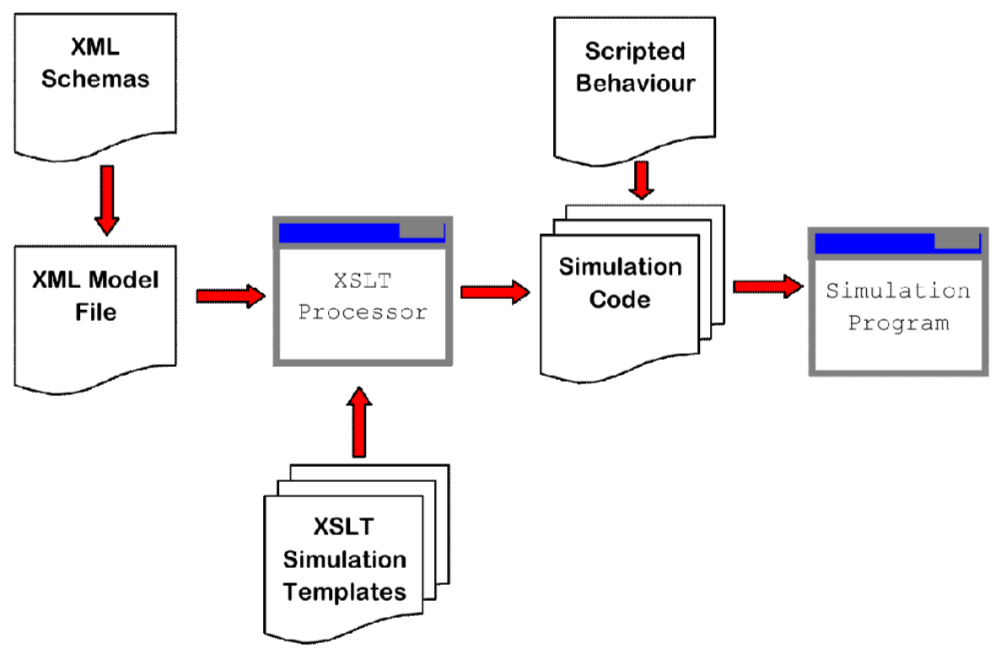
\includegraphics[width=0.5\textwidth]{Appendix/FLAME_Process}
\caption{\gls{FLAME GPU} Development Process (Taken from \cite{flame_simulation})}
\label{fig:flame_dev}
\end{wrapfigure}

Building \gls{FLAME GPU} simulations requires the creation of two artifacts (Fig. \ref{fig:flame_dev}), a structural `XML Model File' which defines the agents in the system and their allowed channels for communication and a C source code file of `Scripted Behaviour' which defines the actual behaviour of agents.

A state-based platform model design is already available- the domain model for the original \gls{MASON} implementation of this simulation.
As \gls{FLAME GPU} uses state machines for each agent type in its implementation, these have been directly implemented into it.

Host cell creation into the system is a work in progress for next \gls{FLAME GPU} release?

Due to time constraints, I have not been able to implement environmental growth.
%This isn't complex to implement within FLAME GPU itself.. a step function could be used to adjust each agent's position.
%Unfortunately at present the FLAME GPU simulation sets the camera in the centre position of the environment bounds- these are determined by the INITIAL position of cells

\subsection{Epsilon}
In the creation of the \gls{FLAME GPU} XML model, I decided to implement a new tool, built using the Epsilon Modelling Framework.
This new tool contains a graphical editor which allows the \gls{FLAME GPU} `XML Model File' to be created diagramatically.
If implemented correctly, the tool should \textit{directly map} the platform model structures into the \gls{FLAME GPU} domain model.
This should significantly improve the model design experience and allow for domain experts to be kept more involved with the simulation creation.
Figure \ref{fig:ppsim_gmf} shows the Peyer's Patch simulation created within this graphical editor. The XML model used for the final simulation was automatically generated from this diagram.

The \gls{evl} has allowed well-formedness constraints to be implemented for the \gls{FLAME GPU} input model.
This should provide intuitive feedback (Fig. \ref{fig:validation_gmf}) in cases where the model may be incorrect, in order to prevent an invalid XML model from being produced.
Quick fixes (Fig. \ref{fig:validation_quickfix_gmf}) have also been implemented to guide the user through easily correcting their invalid model.

One final benefit of this new approach to model generation, is that it makes it far simpler to .
%Hm?

%boolean transition conditions:
%critique allows users to ignore it
%BUT generally, and particularly with biological models like this:
%Transitions.. BETWEEN states require some form of external trigger?

\subsection{Testing}
As the new simulation is a re-engineering of the existing PPSim, it can inherit the validation of the existing simulation.
This requires the new simulation to be demonstrably similar with similar components, behaviours and results.
%is this the case?

Talk about how the model was tested to ensure correctness\\
Mention missing link in (incorrect) model from Kieran's paper 

%Approx 2500 words for results and evalution
\chapter{Results and Evaluation}
\label{results}
%NB.. INTRODUCTION + CONCLUSION MUST MATCH AND REFERENCE EACH OTHER.


\section{Findings}
\subsection{Ease of Use}
"Further work is now being developed with Paul Richmond's \gls{FLAME GPU} group, to enhance the accessibility of \gls{FLAME GPU} for simulation developers."
"This should allow the simulation developer to focus on getting their domain details correct, rather than battling the agent platform."

\subsection{Speed Up}
%Model is too disimilar to Kieran's
The differences between the \gls{MASON} and \gls{FLAME GPU} platforms have meant that it is not trivial to compare them.
%Mention difference between LTo cell division - force resolution step used

%SPEED RESULTS..
%TODO - ensure this is present in introduction
The initial hypothesis of the platform models being comparable is untenable.

%model is abstract from domain already, makes more sense to compare this to domain
Instead, a new hypothesis is that the platform model for the \gls{FLAME GPU} implementation is comparable to the original biological model.

\cite{statistical_tests} could be important for evaluating the performance of \gls{FLAME GPU} against original PPSim

%Approx 1000 words
\section{Conclusion}

\section{Further Work}
\subsection{Hardware Availability}
%OpenGL could be something to discuss here
%dismissed by Phil, but further exploration could be good!
%ANDY is working on this
%Talk about difficulty getting access to the necessary NVIDIA hardware

\subsection{Software Generalisibility}%IS THIS A WORD?
%Expand project for more powerful cell based simulation
%allow access to non-technical users
%flexible modelling
While the use of Epsilon has allowed for domain experts to be kept involved with the model implementation, there is still a final, most technically challenging, stage of the simulation creation where the agent behaviour is programmed.
Further work will need to study agent behaviour in these forms of simulation generally.
The reuse of a previous simulation's implementation of cell division behaviour, has shown that at least some behaviour is common across different simulations.
The power of \gls{mde} is such that this repeated behaviour should be generalised to reduce the time needed and prevent the mistakes that occur during reimplementation of the similar software features.

On top of this, with the current implementation, technical implementation details (layer functions and agent partitioning) have become part of the model.
Ideally these should be extracted from the model implementation and automated.



%explore what the "differences" between the simulations "mean", specifically for PPSim and more generally

\printbibliography
\chapter{Appendix}
\section{Simulation Parameters}


\section{Cell Data Structures}

\section{Other}

\begin{figure}[htp]
\centering
\begin{subfigure}{\textwidth}
\centering
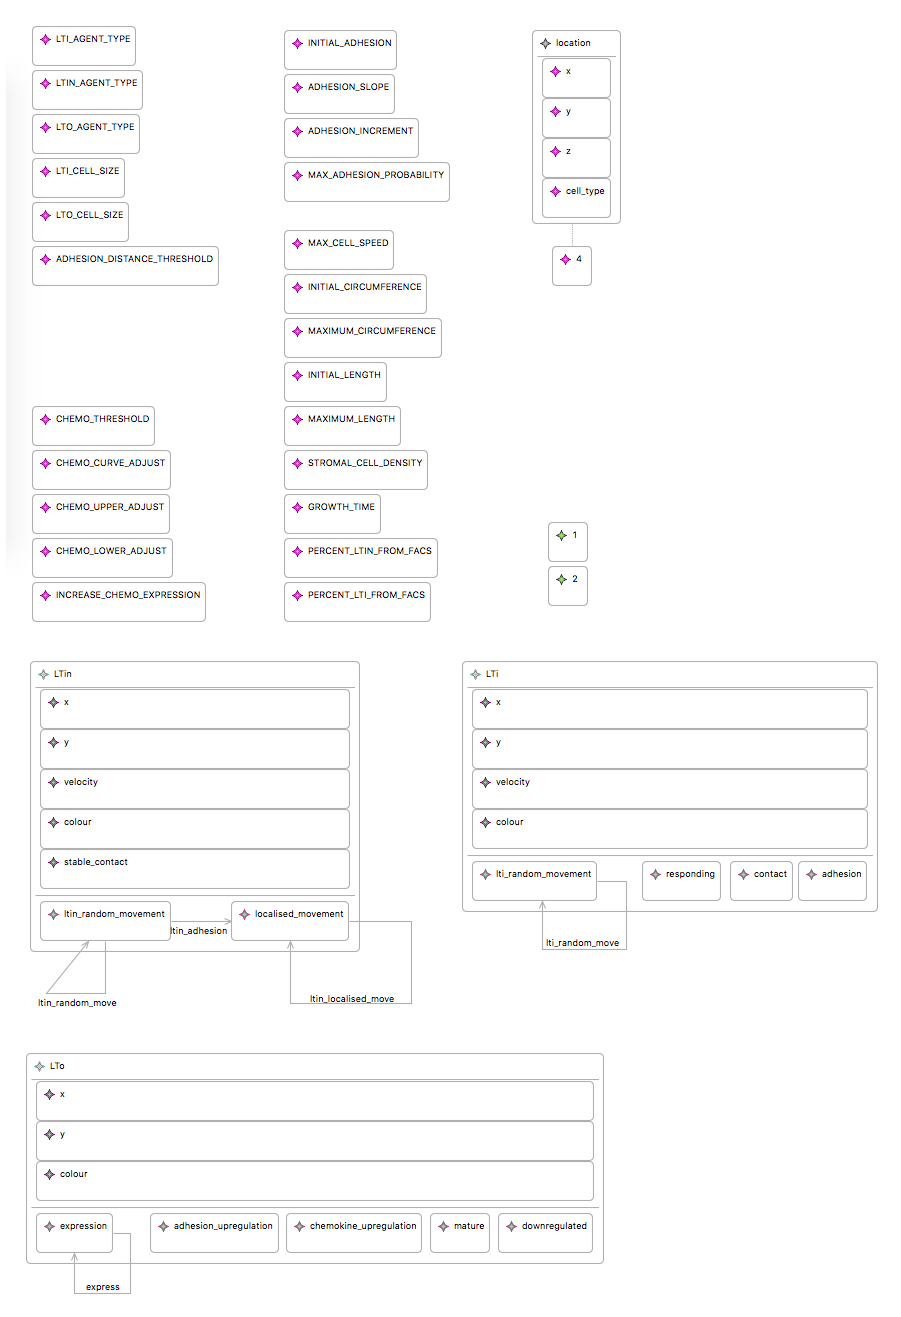
\includegraphics[width=\textwidth]{Appendix/ppsim_gmf}
\caption{Graphically produced \gls{FLAME GPU} Simulation model for Peyer's Patch}
\label{fig:ppsim_gmf}
\end{subfigure}%
\end{figure}

\begin{figure}[htp]\ContinuedFloat
\centering
\begin{subfigure}{\textwidth}
\centering
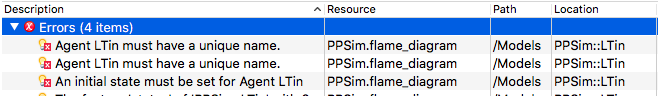
\includegraphics[width=\textwidth]{Appendix/validation_gmf}
\caption{Graphical validation using \gls{evl} constraints}
\label{fig:validation_gmf}
\end{subfigure}

\begin{subfigure}{\textwidth}
\centering
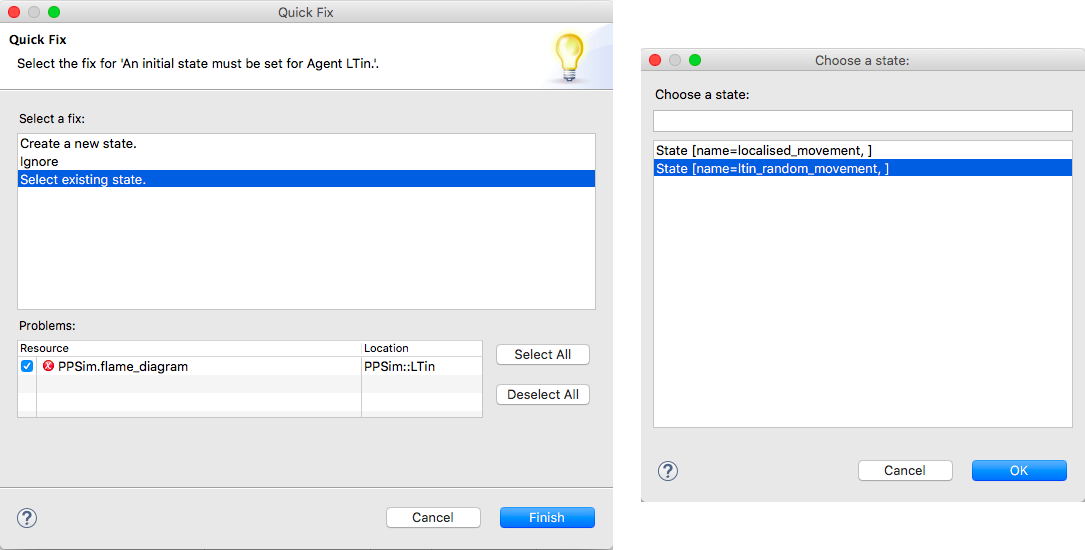
\includegraphics[width=\textwidth]{Appendix/validation_quickfix_gmf}
\caption{Quick fix of invalid model}
\label{fig:validation_quickfix_gmf}
\end{subfigure}%

\caption{Graphical Tool for creating \gls{FLAME GPU} models}
\label{fig:gmf}
\end{figure}
 
\end{document}